\documentclass[pdf]{beamer}
\mode<presentation>{}

\usetheme{Boadilla}
\useoutertheme{split}
\usecolortheme{whale}
\useinnertheme{rounded}
\usepackage{mathptmx}
\usepackage{graphicx}
\usepackage{tikz}
\usetikzlibrary{arrows.meta}
\usepackage{booktabs}
\usepackage{array}
\usepackage{tabularx}
\usepackage{hyperref}

\newcommand{\cellwrap}{%
  \raggedright
  \hyphenpenalty=10000
  \exhyphenpenalty=10000
}
\newcolumntype{Y}{>{\cellwrap\arraybackslash}X}
\newcolumntype{K}{>{\bfseries\cellwrap\arraybackslash}X}
\newcolumntype{L}{>{\cellwrap\arraybackslash}p{2.35cm}}

\title{Desk Buddy}
\subtitle{Project Progress: Problem and Design}
\author{IoT and Applications}
\institute{Hanoi University of Science and Technology}
\date{November 2026}

\begin{document}
\section{Hanoi University of Science and Technology}
\huge
\maketitle
\footnotesize

\begin{frame}{The problem}
\transsplitverticalin
    \begin{block}{A long session at a closed desk}
        \begin{itemize}
            \item Heat, humidity, dim light, heavy air
            \item Easy to miss until focus drops
            \item Breaks are forgotten
        \end{itemize}
    \end{block}
\end{frame}

\begin{frame}{Desk Buddy}
\transsplitverticalout
    \begin{block}{One node for one study desk}
        \begin{itemize}
            \item Senses the desk environment
            \item Sends one reading to the laptop
            \item Shows live numbers and history
            \item Beeps when a break is due
        \end{itemize}
    \end{block}
\end{frame}

\begin{frame}{Scope of this talk}
    \begin{block}{In scope}
        \begin{itemize}
            \item One node: \texttt{node1}
            \item One JSON every 5 seconds
            \item Sensors, MQTT, and a web page
        \end{itemize}
    \end{block}
    \begin{block}{This report}
        \begin{itemize}
            \item Problem, architecture, and choices
            \item Build and measurements come next
        \end{itemize}
    \end{block}
\end{frame}

\begin{frame}{Overall architecture}
    \centering
    \resizebox{0.98\textwidth}{!}{%
    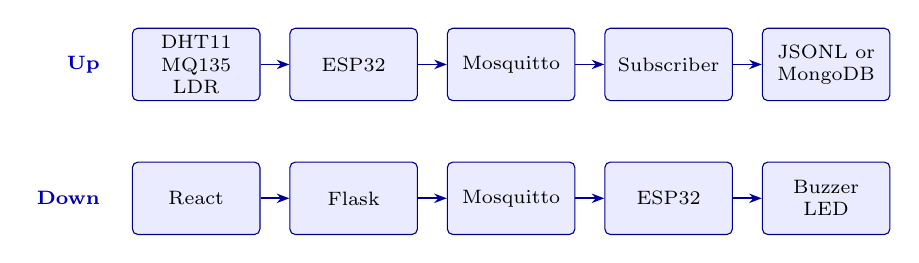
\begin{tikzpicture}[
        box/.style={
            draw=blue!55!black,
            rounded corners=2pt,
            fill=blue!8,
            align=center,
            font=\scriptsize,
            minimum width=1.62cm,
            minimum height=0.92cm,
            inner sep=1.5pt
        },
        arr/.style={-{Stealth[length=1.6mm]}, semithick, blue!60!black},
        lane/.style={font=\scriptsize\bfseries, blue!70!black, anchor=east}
    ]
        \node[lane] at (0.05, 0.95) {Up};
        \node[box] (sens) at (1.15, 0.95) {DHT11\\MQ135\\LDR};
        \node[box] (esp)  at (3.15, 0.95) {ESP32};
        \node[box] (mq)   at (5.15, 0.95) {Mosquitto};
        \node[box] (sub)  at (7.15, 0.95) {Subscriber};
        \node[box] (db)   at (9.15, 0.95) {JSONL or\\MongoDB};
        \draw[arr] (sens) -- (esp);
        \draw[arr] (esp) -- (mq);
        \draw[arr] (mq) -- (sub);
        \draw[arr] (sub) -- (db);

        \node[lane] at (0.05, -0.75) {Down};
        \node[box] (web)  at (1.15, -0.75) {React};
        \node[box] (api)  at (3.15, -0.75) {Flask};
        \node[box] (mq2)  at (5.15, -0.75) {Mosquitto};
        \node[box] (esp2) at (7.15, -0.75) {ESP32};
        \node[box] (act)  at (9.15, -0.75) {Buzzer\\LED};
        \draw[arr] (web) -- (api);
        \draw[arr] (api) -- (mq2);
        \draw[arr] (mq2) -- (esp2);
        \draw[arr] (esp2) -- (act);
    \end{tikzpicture}%
    }

    \vspace{0.45em}
    {\scriptsize The browser talks to Flask only.}
\end{frame}

\begin{frame}{Message and thresholds}
    \begin{columns}[T,onlytextwidth]
        \begin{column}{0.56\textwidth}
            \small
            \textbf{Every 5 seconds}
            \vspace{0.35em}

            \vspace{0.7em}
            \begin{tabular}{@{}ll@{}}
                \toprule
                \textbf{Field} & \textbf{Meaning} \\
                \midrule
                \texttt{tempC} & DHT11, $^\circ$C \\
                \texttt{humidity} & DHT11, \% \\
                \texttt{airRaw} & MQ135, ADC \\
                \texttt{lightRaw} & LDR, ADC \\
                \bottomrule
            \end{tabular}
        \end{column}
        \begin{column}{0.40\textwidth}
            \small
            \textbf{Alert when}
            \vspace{0.8em}

            \begin{tabular}{@{}lr@{}}
                \toprule
                \textbf{Check} & \textbf{Limit} \\
                \midrule
                Hot & $\geq 32^\circ$C \\
                Humid & $\geq 80\%$ \\
                Air & $\geq 1800$ \\
                Dim & $\leq 400$ \\
                \bottomrule
            \end{tabular}

            \vspace{0.8em}
            {\scriptsize ADC stays 0--4095.\\No ppm, no lux.}
        \end{column}
    \end{columns}
\end{frame}

\begin{frame}{Choosing the board}
    \centering
    \small
    \setlength{\tabcolsep}{5pt}
    \setlength{\extrarowheight}{3pt}
    \begin{tabularx}{\textwidth}{@{} K Y Y @{}}
        \toprule
        \textbf{Choice} & \textbf{Why} & \textbf{Alternative} \\
        \midrule
        ESP32 &
        Wi-Fi on the chip. ADC1 still reads while Wi-Fi is on. &
        Arduino Uno: no Wi-Fi. ESP8266: one ADC. Raspberry Pi: too heavy for one node. \\
        \bottomrule
    \end{tabularx}

    \vspace{0.7em}
    {\scriptsize Air and light use GPIO 34 and 35.}
\end{frame}

\begin{frame}{Choosing the sensors}
    \centering
    \small
    \setlength{\tabcolsep}{5pt}
    \setlength{\extrarowheight}{2pt}
    \begin{tabularx}{\textwidth}{@{} L K Y Y @{}}
        \toprule
        \textbf{Measure} & \textbf{Choice} & \textbf{Why} & \textbf{Alternative} \\
        \midrule
        Heat, humidity & DHT11 & Enough for 32$^\circ$C and 80\% & DHT22, BME280 \\
        Air & MQ135, raw ADC & Higher means worse air & Digital ppm sensor \\
        Light & LDR, raw ADC & Brighter means a higher value & BH1750 in lux \\
        Desk alert & Active buzzer and LED & A high pin turns it on & Passive buzzer \\
        \bottomrule
    \end{tabularx}
\end{frame}

\begin{frame}{Choosing the software}
    \centering
    \small
    \setlength{\tabcolsep}{5pt}
    \setlength{\extrarowheight}{2pt}
    \begin{tabularx}{\textwidth}{@{} L K Y Y @{}}
        \toprule
        \textbf{Layer} & \textbf{Choice} & \textbf{Why} & \textbf{Alternative} \\
        \midrule
        Link & MQTT, two topics & Readings up, commands down & HTTP, CoAP \\
        Broker & Mosquitto on the laptop & Runs in the lab & Cloud broker \\
        Services & Subscriber and Flask & The web uses HTTP only & Board writes the database \\
        Store & JSONL now, MongoDB later & Demo still runs offline & MongoDB only \\
        UI & React dashboard & Live view in the browser & Serial monitor \\
        \bottomrule
    \end{tabularx}
\end{frame}

\begin{frame}{Where we are}
    \begin{block}{Started}
        \begin{itemize}
            \item Contract is fixed: topics, fields, limits
            \item Laptop path runs with the simulator
        \end{itemize}
    \end{block}
    \begin{block}{Next}
        \begin{itemize}
            \item Flash the firmware
            \item Read the real sensors
            \item Fill the measurement table
        \end{itemize}
    \end{block}
\end{frame}

\begin{frame}{Summary}
    \begin{itemize}
        \item One desk node for comfort and breaks
        \item ESP32, DHT11, MQ135, LDR
        \item MQTT on the laptop, then Flask and React
    \end{itemize}
\end{frame}

\begin{frame}
    \centering
    \vspace{1cm}
    \huge{Thank you for listening!!}
\end{frame}

\end{document}
